\documentclass[a4paper, 10pt]{article}

\usepackage{global-macros}
\usepackage{fullpage}
\usepackage{sectsty}

\allsectionsfont{\large\sffamily}

\title{{\Large\bfseries\sffamily Bayesian Statistics --- Assignment 2} \\ \large\sffamily On the Bayesian Lasso}
\author{\normalsize Caio Peixoto}
\date{\normalsize\today}

\begin{document}

\maketitle

\tableofcontents

\section{LASSO regression and the Laplace prior}
In\footnote{Corresponds to items a) and b).} this work we will study the usual linear regression model, given by 
\begin{equation}
    \by \mid \mu, \betabold, \bX, \sigma^2 \sim \Normal(\mu \ones_{ n } +  \bX \betabold, \sigma^2 \eye_n)
    \label{eq: likelihood}
,\end{equation}
where $ \bX \in \R^{n \times p}, \betabold \in \R^{ p }, \mu \in \R $, $ \ones_{ n } $ denotes the vector in $ \R^{ n } $ with all coordinates set to $ 1 $ and $ \eye_{ n } $ denotes the $ n $-dimensional identity matrix.
The goal is to conduct inference on $ \mu, \betabold $ and $ \sigma^2 $, and we will follow the Bayesian approach in \cite{parkcasella2008bayesianlasso}.

In \cite{tibshirani1994lasso}, the author presented an estimator for $ \betabold $ and $ \mu $, called the LASSO\footnote{\emph{Least absolute shrinkage selection operator.}}, with the following definition:
\begin{equation}
    ( \hat{ \betabold }_{ \lasso }, \hat{ \mu }_{ \lasso } )
    = \argmin_{ \norm{ \betabold }_{ 1 } \leq t, \mu \in \R } \ \norm{\by - \mu \ones_{ n } - \bX \betabold}_2^2
    \label{eq: lasso constrained}
,\end{equation}
where $ t > 0 $ is a tuning parameter.
His goal was to address two of the main problems of the usual OLS estimator, which does not include the $ L^{ 1 } $ norm constraint: \emph{high variance}, which lowers prediction accuracy, and \emph{lack of interpretability}, particularly when the number of predictors is high.
The effect produced by the $ L^1 $ constraint is the shrinkage of the overall coefficient magnitude and, more importantly, the collapse of the less important coefficients to exactly $ 0 $.
This effect introduces bias in the estimation, but the gain in variance is enough to improve predictive performance.
Furthermore, it provides a principled way to perform variable selection, by discarding the variables whose coefficients were collapsed to $ 0 $.

One might wonder what is special about the $ L^1 $ norm, since this collapsing behavior is not observed for the Ridge estimator, which uses $ L^2 $ constraint instead of $ L^1 $.
It turns out the reason is geometric.
The $ L^1 $ ball in $ \R^{ p } $ has sharp edges and vertices, in contrast with the smooth surface of the $ L^2 $ ball.
When solving problem (\ref{eq: lasso constrained}), the solution will often be located on an edge of the $ L^1 $ ball of radius $ t $.
Along these edges, one or more coefficients are exactly zero, which produces the collapsing effect.

Although the methodology in \cite{tibshirani1994lasso} is classical, in Section 5 the authors point out that problem (\ref{eq: lasso constrained}) is equivalent to MAP estimation when employing a Laplace prior.
To see this, note that the constrained optimization problem is equivalent to the following regularized version:
\begin{equation*}
    \argmin_{ \betabold \in \R^{ p }, \mu \in \R } \norm{ \by - \mu \ones_{ n } - \bX \betabold }_{ 2 }^{ 2 } + \lambda \norm{ \betabold }_{ 1 }
,\end{equation*}
where $ \lambda $ depends on $ t $.
Much like the squared Euclidean norm in the objective corresponds to the normal likelihood, the $ L^1 $ norm can be seen as the log of the kernel of the Laplace distribution.
Hence, the LASSO is the MAP estimator when the prior for $ \betabold $ is chosen as
\begin{equation*}
    \pi ( \betabold ) = \left( \frac{ \lambda }{ 2 } \right)^n \exp \left\{ - \lambda \norm{ \betabold }_{ 1 } \right\}
.\end{equation*}
Expanding upon this observation, in \cite{parkcasella2008bayesianlasso} the authors discuss a Bayesian formulation for LASSO regression by employing the following joint prior on $ \betabold $ and $ \sigma $:
\begin{align}
    \begin{split}
        \pi ( \sigma^2 ) &\propto \frac{ 1 }{ \sigma^2 } \cdot \ind \{ \sigma^2 > 0 \}, \\
        \pi ( \betabold \mid \sigma^2 ) &= \left( \frac{ \lambda }{ 2 \sqrt{ \sigma^2 } } \right)^{ n } \exp \left\{ - \frac{ \lambda }{ \sqrt{ \sigma^2 } } \norm{ \betabold }_{ 1 } \right\},
    \end{split}
    \label{eq: conditional laplace prior}
\end{align}
where $ \lambda $ is a hyperparameter which can be given a hyperprior or be estimated using marginal maximum likelihood methods.
The choice for a Laplace prior for $ \betabold $ is necessary to recover the LASSO estimator as the MAP.
With a normal prior, for instance, the MAP would become the Ridge regression estimator.
This conditional structure in the prior is justified in \cite{parkcasella2008bayesianlasso} by a computational argument: without it, the posterior may exhibit multimodality, which can pose difficulties for MCMC sampling schemes such as the Gibbs sampler.
From a statistical perspective, this prior encapsulates the idea that the larger $ \sigma^2 $ is, the less informative the prior on $ \betabold $ should be.
This makes \emph{some} sense, since, for more spread out $ y $ values, we would like the prior not to be as restrictive and not to ``get in the way'' of the likelihood.
On another note, it would also be reasonable not to assume $ \betabold $ and $ \sigma^2 $ depend on each other in any way a \emph{priori}.
Anyway, since we are following the methodology of \cite{parkcasella2008bayesianlasso}, our prior of choice will be (\ref{eq: conditional laplace prior}).

The main motivation for this Bayesian formulation is the already mentioned fact that the LASSO estimator is recovered as the MAP.
However, Bayesian estimation goes far beyond maximizing the posterior, and one might wonder if other forms of inference based on the prior (\ref{eq: conditional laplace prior}) exhibit shrinkage-like properties.
This, among other things, is what we will investigate in the following sections.
Apart from the usual advantages of having a full probability distribution describing our belief about the parameters, it is not clear if this Bayesian approach does what we might desire it to do, e.g., produce credibility intervals which include $ 0 $ for the irrelevant covariates and exclude it for the relevant ones.
In fact, there are statisticians which assert that the Bayesian LASSO simply \emph{does not work}, as can be seen, for instance, in \cite{simpson2021}.
Simpson's argument is that the prior (\ref{eq: conditional laplace prior}) either shrinks \emph{almost all} parameters to $ 0 $, or does not produce \emph{any shrinkage at all}.

% \begin{itemize}
%     \item Introduce notation for linear regression;
%     \item Explain the Lasso regularization;
%     \item Explain why the L1 norm produces shrinkage;
%     \item Show how the LASSO estimator is the MAP estimator when using the Laplace prior;
%     \item Explain the conditional structure of the Laplace prior;
%     \item Comment on possible advantages of having a full probability distribution for the parameters;
%     \item Talk about possible disadvantages of using the Laplace prior, allude to excessive shrinkage in the experiments;
% \end{itemize}

\section{The Gibbs sampler}
In\footnote{Corresponds to items c) and d).} \cite{parkcasella2008bayesianlasso}, the authors propose a Gibbs sampler to draw samples from the posterior.
This sampler uses the following decomposition of the Laplace distribution: if $s \sim \Exp(a^2 / 2)$\footnote{This is the \emph{rate} parameter} and $ z \mid s \sim \Normal(0, s) $, then, marginally, $ z \sim \Laplace(a) $, that is,
\begin{equation*}
    p ( z ) = \frac{ a }{ 2 } \exp \{ - a \abs{ z } \}
.\end{equation*}
Using this decomposition, one may rewrite the model given by (\ref{eq: likelihood}) and (\ref{eq: conditional laplace prior}) with auxiliary variables $ \tau_{ 1 }^2, \dots, \tau_{ p }^2 $:
\begin{align*}
    \by \mid \mu, \betabold, \bX, \sigma^2 &\sim \Normal(\mu \ones_{ n } +  \bX \betabold, \sigma^2 \eye_n), \\
    \betabold \mid \sigma^2, \tau_{ 1 }^2, \dots, \tau_{ p }^2 &\sim \Normal (\zeros_{ p }, \sigma^2 \bD_{ \tau }), \\
    \bD_{ \tau } &= \diag (\tau_{ 1 }^2, \dots, \tau_{ p }^2), \\
    \tau_{ i }^2 &\iid \Exp(\lambda^2 / 2),
\end{align*}
and $ \sigma^2 $ is distributed independently of $ \tau_{ 1:p }^2 $ according to a distribution $ \pi $ with positive support, while $ \mu $ is given an independent, flat, prior.
Park and Casella chose to use $ \pi \propto \frac{ 1 }{ \sigma^2 } \ind \{ \sigma^2 > 0 \} $, but, as they mentioned in \cite{parkcasella2008bayesianlasso}, any inverse-gamma prior could be used without affecting conjugacy.
This is a way to introduce subjective knowledge about $ \sigma^2 $ to the prior.
It is necessary to introduce the auxiliary variables $ \tau_{ 1 }^2, \dots, \tau_{ p }^2 $ because the $ L^1 $ norm which appears inside the exponential in the Laplace distribution makes the full conditional of $ \betabold $ hard to sample from.
With this new hierarchical structure, the full conditional of $ \betabold $ is multivariate normal, while that of $ \sigma^2 $ and $ 1/\tau_{ i }^2 $ are inverse gamma and inverse Gaussian, respectively.
Of course, this is only needed if one is interested in fully exploring the posterior distribution.
If all one desires is to compute the MAP, then it is best to go back to the prior in (\ref{eq: conditional laplace prior}) and use any available package to obtain the LASSO estimator.

The intercept parameter, $ \mu $, is only related to the location of $ \by $, and, thus, does not contain any information on which covariates are relevant and which are not.
If the goal of the data analyst is only to analyze the effect of each covariate on the outcome, there is no reason to conduct inference on (and, hence, sample from) the intercept $ \mu $.
It can be easily marginalized from the joint distribution of data and parameters, and this was the rout taken in \cite{parkcasella2008bayesianlasso}.
The authors mention that, should one desire to sample from $ \mu $, its full conditional is normal with mean $ \bar{ \by } $ and variance $ \sigma^2/n $.


% \begin{itemize}
%     \item Explain the sampling hierarchy suggested by Park and Casella.
%     \item Modify the hierarchy to facilitate MAP estimation;
%     \item Discuss how one should include information about the measurement noise parameter?
%     \item Discuss why marginalize $\mu$ in the computation and when that is and is not desirable;
%     \item Show how to recover inferences about $ \mu  $ in the marginalized case.
% \end{itemize}

\section{But can it actually shrink?}
In\footnote{Corresponds to item e).} this section, we will investigate the shrinking properties of the Bayesian LASSO using the artificial data scenarios in presented in the Section 7.2 of \cite{tibshirani1994lasso}.
All the scenarios consist of generating $ n $ samples from the model in (\ref{eq: likelihood}), where the lines of $ \bX $ are independent samples from a multivariate normal distribution.
For the prior distribution, we employed the prior in (\ref{eq: conditional laplace prior}), with an additional $ \distgamma (\delta, r) $ prior\footnote{Here, $ \delta $ and $ r $ are the \emph{shape and rate} parameters, respectively.} on $ \lambda^2 $ (not $\lambda$), as suggested in Section 3.2 of \cite{parkcasella2008bayesianlasso}.
We specified a weakly-informative prior by choosing $ \delta = 1.0 $ and $ r = 0.1 $.
The sampling scheme we chose was NUTS-HMC, utilized through \texttt{Stan} \cite{stan2024}.
For each dataset, we sampled from $ 5 $ chains, using $ 1000 $ warm-up samples and $ 10 000 $ samples from (hopefully) the posterior.
On a last note, we also standardized the columns of $ \bX $ to have mean $ 0 $ and variance $ 1 $.
This is a good practice also employed in \cite{parkcasella2008bayesianlasso}, as it puts all covariates in the same scale.
If one of the betas was much smaller than the other ones simply because of the larger scale of the corresponding covariate, then it might be incorrectly shrunk to $ 0 $ by the LASSO regression.

\subsection*{Scenario 1}

For this scenario, the parameters were
\begin{align*}
    \betabold &= (3, 1.5, 0, 0, 2, 0, 0, 0) \\
    \sigma &= 3
.\end{align*}
The correlation between $ x_{ i } $ and $ x_{ j } $ was set to $ \rho^{ \abs{ i - j } } $, with $ \rho = 0.5 $.
All $ (x_{ i })_{ 1 \leq i \leq 8 } $ had mean $ 0 $.
We studied two sample sizes: $ n = 20 $ and $ n = 100 $.

Effective sample size and $ \hat{ R } $ statistics are in Table \ref{tab: Eff and Rhat scenario 1}.
We can see that, for both values of $ n $, the $ \hat{ R } $ values are very close to one, indicating that we are indeed sampling from the posterior.
The effective sample sizes are also quite high, which allows us to trust the credibility intervals computed from these samples.
\begin{table}[htb]
    \centering
    \begin{tabular}{lrr}
& $ n = 20 $ & \\
\toprule
 & N\_Eff & R\_hat \\
\midrule
lp\_\_ & 15200.000000 & 1.000000 \\
mu & 47660.000000 & 1.000000 \\
beta[1] & 31305.000000 & 1.000000 \\
beta[2] & 30485.000000 & 1.000000 \\
beta[3] & 33833.000000 & 1.000000 \\
beta[4] & 39068.000000 & 1.000000 \\
beta[5] & 36640.000000 & 0.999900 \\
beta[6] & 35091.000000 & 1.000000 \\
beta[7] & 33731.000000 & 1.000000 \\
beta[8] & 35182.000000 & 1.000000 \\
sigma & 32499.237400 & 1.000100 \\
lambda & 36077.141000 & 1.000000 \\
\bottomrule
\end{tabular}

    \quad
    \begin{tabular}{lrr}
& $ n = 100 $ &
\toprule
 & N\_Eff & R\_hat \\
\midrule
lp\_\_ & 19470.000000 & 1.000000 \\
mu & 54950.000000 & 1.000000 \\
beta[1] & 41583.000000 & 1.000000 \\
beta[2] & 38976.000000 & 1.000000 \\
beta[3] & 32296.000000 & 1.000000 \\
beta[4] & 35541.000000 & 0.999900 \\
beta[5] & 36941.000000 & 1.000000 \\
beta[6] & 34982.000000 & 1.000000 \\
beta[7] & 31183.000000 & 1.000000 \\
beta[8] & 33972.000000 & 1.000000 \\
sigma & 45289.799000 & 1.000000 \\
lambda & 44630.841000 & 1.000000 \\
\bottomrule
\end{tabular}

    \caption{Effective sample size and $ \hat{ R } $ statistics for Scenario 1, with four significant digits.}
    \label{tab: Eff and Rhat scenario 1}
\end{table}
In order to further assess chain mixing, we show trace plots of the parameters in Figure \ref{fig: traceplots scenario 1}.
From them, we can see that the chains are generally well mixed for both dataset sizes.
\begin{figure}[htb]
    \begin{center}
        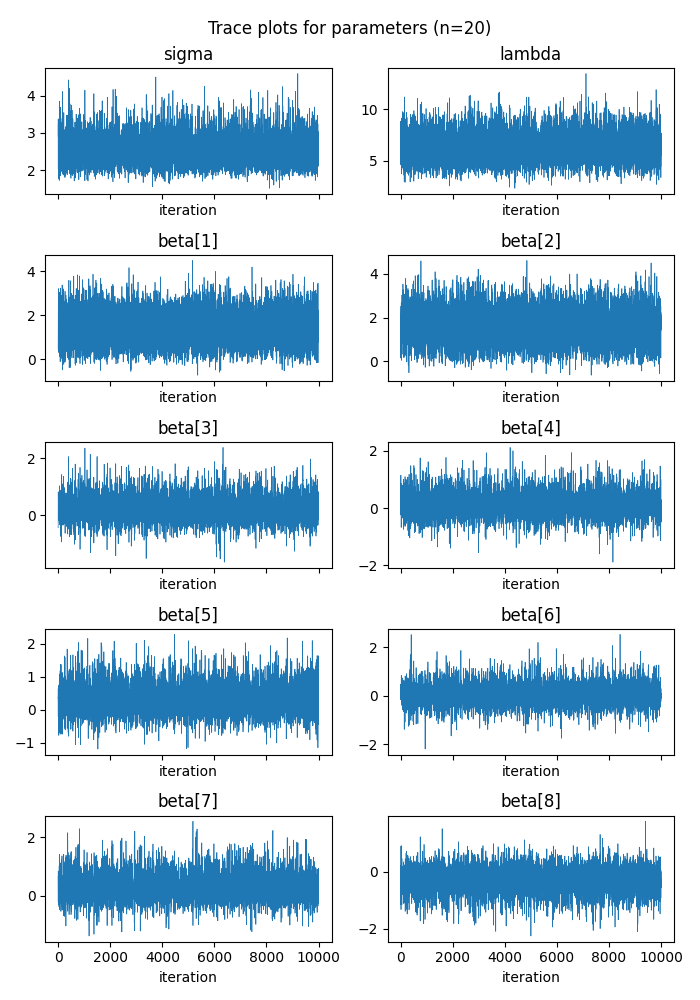
\includegraphics[height=.4\textheight]{../outputs/artificial_scenarios_n=20/scenario_1/traceplots.png}
        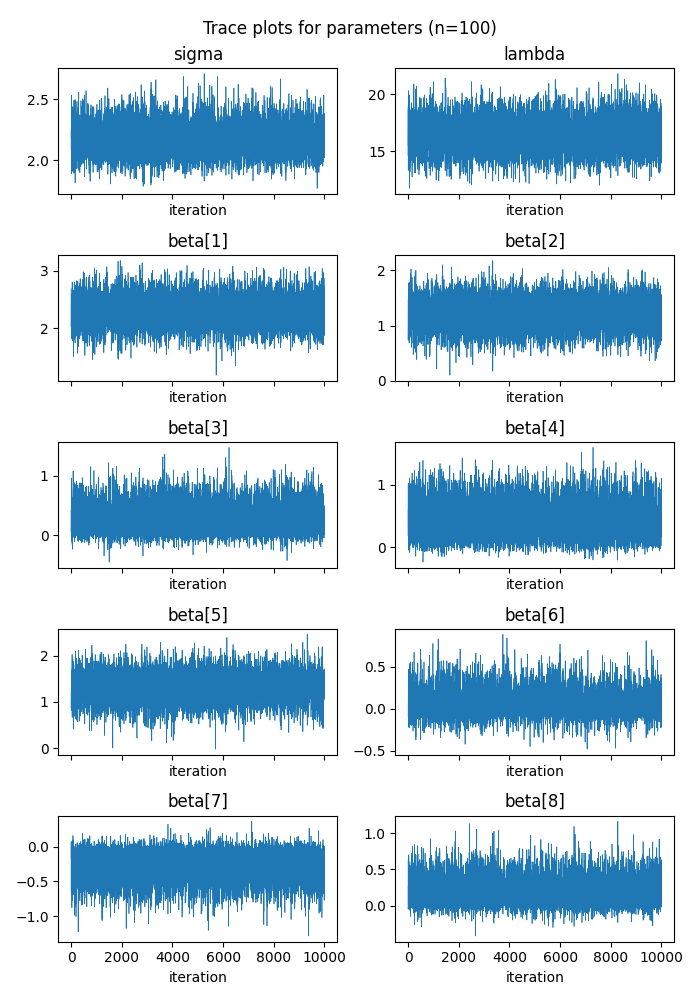
\includegraphics[height=.4\textheight]{../outputs/artificial_scenarios_n=100/scenario_1/traceplots.png}
    \end{center}
    \caption[Trace plots for the parameters in Scenario 1.]{Trace plots for the parameters in Scenario 1. Each plot is from one of the 5 chains, chosen randomly and uniformly.}
    \label{fig: traceplots scenario 1}
\end{figure}
As a final diagnostic, we also conducted a posterior predictive check, whose results are in Figure \ref{fig: posterior predictive check scenario 1}.
To do this, for each sample from the posterior, we sampled $ \by $ according to (\ref{eq: likelihood}) and plotted a histogram of the coordinates.
The actual data is included for comparison.
We can see that there is little resemblance between actual and simulated data for $ n = 20 $, but the situation is better for $ n = 100 $.
This can be due to the large variance ($ \sigma^2 = 9 $) in the data generating process, which makes it hard to extract information from datasets with few samples.
\begin{figure}[htb]
    \begin{center}
        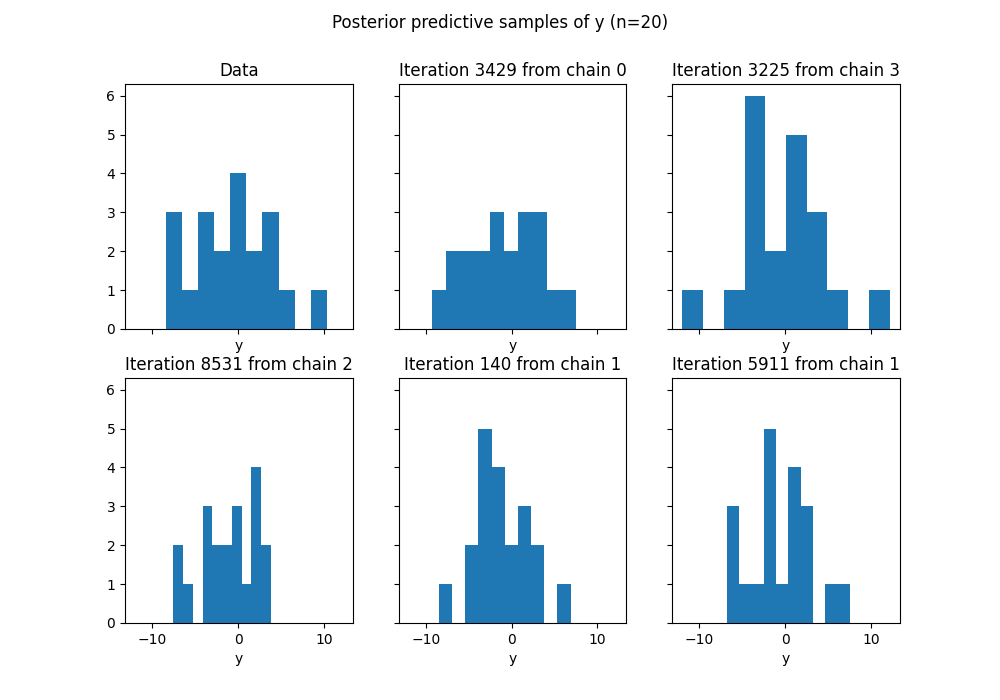
\includegraphics[height=.5\textwidth]{../outputs/artificial_scenarios_n=20/scenario_1/posterior_predictive_check.png}
        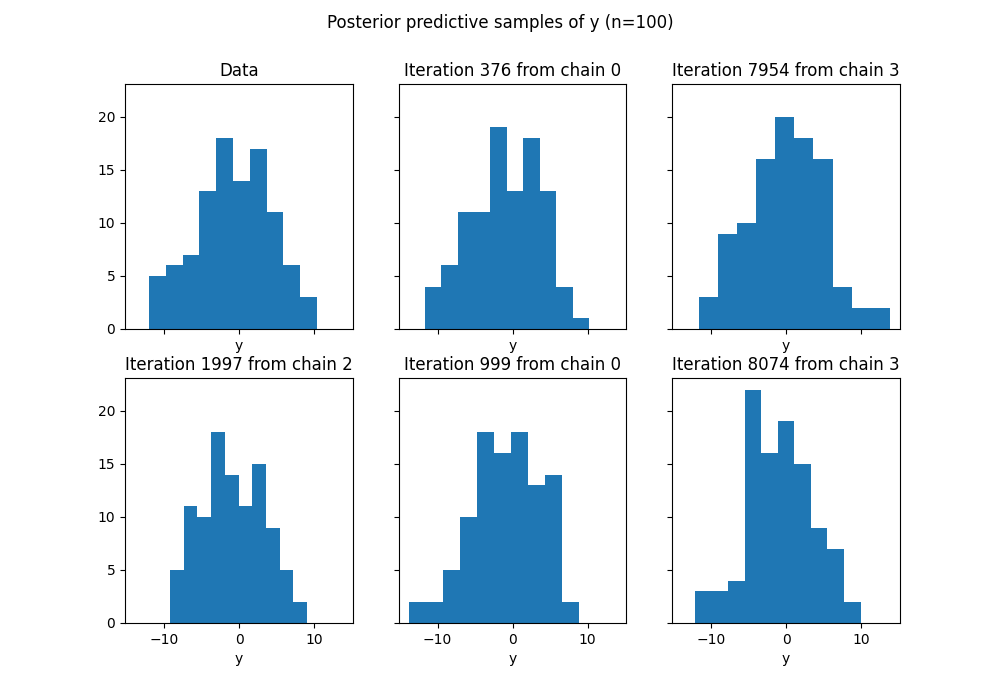
\includegraphics[height=.5\textwidth]{../outputs/artificial_scenarios_n=100/scenario_1/posterior_predictive_check.png}
    \end{center}
    \caption[Posterior predictive checks for Scenario 1.]{Posterior predictive checks for Scenario 1. The parameters corresponding to these $ 8 $ (for each $ n $) simulated values from $ \by $ were randomly and uniformly chosen across all samples from the posterior.}
    \label{fig: posterior predictive check scenario 1}
\end{figure}

To assess shrinkage, we computed $ 95\% $ credibility intervals using the $ 2.5\% $ and $ 97.5\% $ quantiles of the $ 50 000 $ posterior samples.
These are shown in Figure
\begin{figure}[htb]
    \begin{center}
        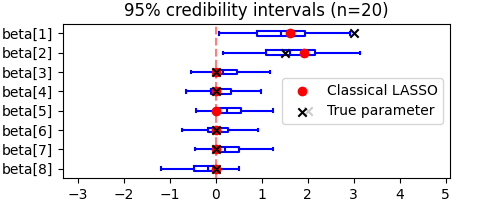
\includegraphics[width=.6\textwidth]{../outputs/artificial_scenarios_n=20/scenario_1/credibility_intervals.png}
        \vspace{1cm}
        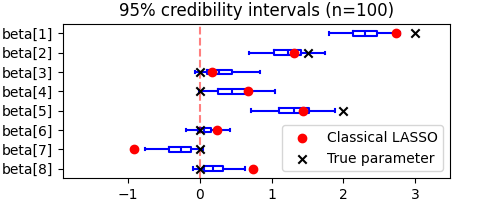
\includegraphics[width=.6\textwidth]{../outputs/artificial_scenarios_n=100/scenario_1/credibility_intervals.png}
    \end{center}
    \caption[95\% credibility intervals for Scenario 1.]{95\% credibility intervals for Scenario 1. The red crosses are the true parameter values. The vertical red line corresponds to $ x = 0 $.}
    \label{}
\end{figure}

For each scenario:
\begin{itemize}
    \item Show table with Stan summary;
    \item Show trace plots of chains for all parameters;
    \item Show prior and posterior predictive distributions;
    \item Show graph with 95\% confidence intervals for all parameters;
\end{itemize}

\section{Choosing $\lambda$}
The\footnote{Corresponds to item f).}

\section{The ``Huberised'' LASSO}
The\footnote{Corresponds to item g).}

\printbibliography

\end{document}